\clearpage

\section{Assignment 2}

The training set (\texttt{data\_train.mat}) has 577 samples with five features $x_1$--$x_5$; \texttt{label\_train.mat} gives
each sample's class as $+1$ or $-1$. There are 301 samples labelled $+1$ and 276 labelled $-1$, and no missing values. The test
set (\texttt{data\_test.mat}) has 23 unlabelled samples. Below, class $\omega_1$ means label $+1$ and class $\omega_2$ means
label $-1$.

\subsection{Fisher linear discriminant classifier}

Fisher's method looks for a direction $\mathbf{w}$ such that, once every sample is projected onto it
($y = \mathbf{w}^T\mathbf{x}$), the two projected class means are far apart while each class's projected samples stay close
together. It maximises the Fisher criterion
\[
J(\mathbf{w}) = \frac{(\tilde{m}_1-\tilde{m}_2)^2}{\tilde{s}_1^2+\tilde{s}_2^2}
= \frac{\mathbf{w}^T S_B \mathbf{w}}{\mathbf{w}^T S_W \mathbf{w}},
\]
where $\tilde{m}_i$ is the projected class mean, $\tilde{s}_i^2 = \sum_{y\in\omega_i}(y-\tilde{m}_i)^2$ is the projected
within-class \emph{scatter} (a sum of squares, not divided by a count),
$S_B = (\mathbf{m}_1-\mathbf{m}_2)(\mathbf{m}_1-\mathbf{m}_2)^T$ is the between-class scatter matrix, and $S_W$ is the
within-class scatter matrix defined below.

The class mean vectors are $\mathbf{m}_i = (1/N_i)\sum_{\mathbf{x}\in\omega_i}\mathbf{x}$, with $N_1 = 301$ and $N_2 = 276$:
\begin{align*}
\mathbf{m}_1 &= (-0.0418,\, 0.0671,\, -0.0540,\, 0.0912,\, -0.0147)^T, \\
\mathbf{m}_2 &= (1.0428,\, 2.0623,\, 0.9408,\, 1.2551,\, 1.6047)^T, \\
\mathbf{m}_1-\mathbf{m}_2 &= (-1.0846,\, -1.9952,\, -0.9947,\, -1.1639,\, -1.6194)^T .
\end{align*}

The within-class scatter of each class is
$S_i = \sum_{\mathbf{x}\in\omega_i}(\mathbf{x}-\mathbf{m}_i)(\mathbf{x}-\mathbf{m}_i)^T$, again a scatter and not divided by
$N_i$, and $S_W = S_1 + S_2$:

\begin{table}[htbp]
\centering
\footnotesize
\caption{Within-class scatter matrix $S_W$ ($5\times 5$, symmetric).}
\begin{tabular}{@{}rrrrr@{}}
\toprule
$568.11$ & $16.99$ & $-0.13$ & $21.12$ & $-9.17$ \\
$16.99$ & $567.74$ & $-17.44$ & $28.77$ & $-8.01$ \\
$-0.13$ & $-17.44$ & $540.03$ & $15.81$ & $-8.42$ \\
$21.12$ & $28.77$ & $15.81$ & $604.84$ & $-8.36$ \\
$-9.17$ & $-8.01$ & $-8.42$ & $-8.36$ & $637.31$ \\
\bottomrule
\end{tabular}
\end{table}

$S_W$ is non-singular, being strongly diagonally dominant, so the system $S_W\mathbf{w} = \mathbf{m}_1-\mathbf{m}_2$ has a
unique solution and can be solved directly. The script does that by Gaussian elimination, without forming an explicit inverse.

Setting the gradient of $J(\mathbf{w})$ to zero gives the generalised eigenvalue problem
$S_B\mathbf{w} = \lambda S_W\mathbf{w}$. Because $S_B\mathbf{w}$ always points along $\mathbf{m}_1-\mathbf{m}_2$, and the length
of $\mathbf{w}$ does not change the decision, the solution is
\[
\mathbf{w} = S_W^{-1}(\mathbf{m}_1-\mathbf{m}_2)
= 10^{-3}\times(-1.7860,\, -3.4729,\, -1.9467,\, -1.6826,\, -2.6581)^T .
\]
The entries are small only because $S_W$ is a sum over 577 samples; scaling $\mathbf{w}$ and $w_0$ by the same positive
constant gives the same decision. This orientation $(\mathbf{m}_1-\mathbf{m}_2)$ places class $\omega_1$ on the positive side of
the boundary. At this $\mathbf{w}$, $J(\mathbf{w}) = 0.0171$: the projected means are
$\tilde{m}_1 = -0.168\times10^{-3}$ and $\tilde{m}_2 = -17.233\times10^{-3}$
($8.53\times10^{-3}$ either side of the boundary), and the projected within-class standard deviations are $5.19\times10^{-3}$ and
$5.72\times10^{-3}$. The second class is the more spread out after projection, which is consistent with its larger share of the
training errors (26 against 13).

Fisher's criterion fixes only the direction, so the bias is a separate convention. The one I used puts the boundary through the
midpoint of the two class means, i.e. $g((\mathbf{m}_1+\mathbf{m}_2)/2) = 0$:
\[
w_0 = -\mathbf{w}^T\frac{\mathbf{m}_1+\mathbf{m}_2}{2}
= -\frac{(-0.1678)+(-17.2331)}{2}\times10^{-3} = 8.7005\times10^{-3} .
\]
The midpoint assumes equal priors and equal misclassification costs. It is a choice rather than a tuned threshold: tuning the
bias on the training data could shrink the 26 errors against 13, and nothing here is tuned on the test set.

Weights and bias together then give the discriminant function
\begin{align*}
g(\mathbf{x}) &= \mathbf{w}^T\mathbf{x} + w_0 \\
&= 10^{-3}\times\bigl(-1.7860\,x_1 - 3.4729\,x_2 - 1.9467\,x_3 - 1.6826\,x_4 - 2.6581\,x_5 + 8.7005\bigr).
\end{align*}
If $g(\mathbf{x}) > 0$ the sample goes to $\omega_1$ (label $+1$), otherwise to $\omega_2$ (label $-1$), so an exact tie
$g(\mathbf{x}) = 0$ falls to $\omega_2$. The boundary $g(\mathbf{x}) = 0$ is a hyperplane in the 5-dimensional feature space. On
the 577 training samples the classifier is 93.2\% correct:

\begin{table}[htbp]
\centering
\footnotesize
\caption{Fisher discriminant confusion matrices on the 577 training samples (rows = true label, columns = predicted label).}
\begin{tabular}{@{}ccccc@{}}
\toprule
\multirow{2}{*}{True} & \multicolumn{2}{c}{Resubstitution} & \multicolumn{2}{c}{Leave-one-out} \\
\cmidrule(lr){2-3}\cmidrule(lr){4-5}
 & $+1$ & $-1$ & $+1$ & $-1$ \\
\midrule
$+1$ & 288 & 13 & 287 & 14 \\
$-1$ & 26 & 250 & 26 & 250 \\
\bottomrule
\end{tabular}
\end{table}

Resubstitution gives $538/577 = 93.24\%$ and leave-one-out $537/577 = 93.07\%$. With only six free parameters (five weights and
a bias) the two agree closely, the single extra leave-one-out error being in class $\omega_1$.

\subsection{Predicted class labels of the test data}

Test sample 1, $\mathbf{x} = (0.0058,\, 1.5626,\, 0.4474,\, 2.0909,\, 0.8973)^T$, has products $w_jx_j$
($\times 10^{-3}$) of $-0.0103$, $-5.4267$, $-0.8709$, $-3.5181$ and $-2.3852$, so
$\mathbf{w}^T\mathbf{x} = -12.2113\times10^{-3}$ and
$g(\mathbf{x}) = (-12.2113+8.7005)\times10^{-3} = -3.511\times10^{-3} < 0$, which gives label $-1$.

\begin{table}[htbp]
\centering
\footnotesize
\caption{Discriminant values and predictions for the 23 test samples. Inputs are shown rounded to 3 decimal places;
$g(\mathbf{x})$ is computed from the unrounded data.}
\begin{tabular}{@{}rrrrrrrr@{}}
\toprule
Test \# & $x_1$ & $x_2$ & $x_3$ & $x_4$ & $x_5$ & $g(\mathbf{x})\times10^{3}$ & Predicted label \\
\midrule
1 & 0.006 & 1.563 & 0.447 & 2.091 & 0.897 & $-3.511$ & $\mathbf{-1}$ \\
2 & 1.229 & 1.440 & 0.878 & $-0.119$ & 1.469 & $-3.907$ & $\mathbf{-1}$ \\
3 & 2.340 & 0.968 & $-0.342$ & 2.123 & 0.848 & $-4.002$ & $\mathbf{-1}$ \\
4 & 0.232 & 1.969 & 0.359 & 1.583 & 0.804 & $-4.051$ & $\mathbf{-1}$ \\
5 & 0.458 & 2.233 & $-0.623$ & 1.563 & 0.725 & $-3.217$ & $\mathbf{-1}$ \\
6 & 0.697 & 2.393 & $-1.182$ & 0.833 & 1.532 & $-4.028$ & $\mathbf{-1}$ \\
7 & $-0.174$ & 1.710 & 0.617 & 1.233 & 1.335 & $-3.750$ & $\mathbf{-1}$ \\
8 & 1.171 & 1.300 & 0.185 & 1.828 & 0.785 & $-3.428$ & $\mathbf{-1}$ \\
9 & 2.065 & 0.830 & 0.279 & 1.601 & 1.032 & $-3.854$ & $\mathbf{-1}$ \\
10 & 0.835 & 0.930 & $-0.577$ & 0.649 & 0.183 & 3.525 & $\mathbf{+1}$ \\
11 & 0.495 & 1.605 & 0.416 & 0.847 & $-1.551$ & 4.132 & $\mathbf{+1}$ \\
12 & 1.534 & 1.067 & $-1.991$ & 1.037 & 0.334 & 3.499 & $\mathbf{+1}$ \\
13 & $-0.479$ & 0.371 & 0.941 & 0.398 & 0.893 & 3.391 & $\mathbf{+1}$ \\
14 & $-0.633$ & $-0.623$ & $-0.492$ & 1.442 & 2.314 & 4.372 & $\mathbf{+1}$ \\
15 & $-1.046$ & 1.920 & $-0.969$ & 0.236 & 0.588 & 3.827 & $\mathbf{+1}$ \\
16 & 1.620 & 1.127 & 1.491 & $-1.297$ & $-0.861$ & 3.459 & $\mathbf{+1}$ \\
17 & 1.296 & 1.226 & $-0.415$ & $-0.447$ & 0.163 & 3.253 & $\mathbf{+1}$ \\
18 & $-0.107$ & 0.992 & $-0.598$ & 0.024 & 1.206 & 3.363 & $\mathbf{+1}$ \\
19 & $-1.002$ & 1.383 & 0.837 & $-0.486$ & 0.621 & 3.224 & $\mathbf{+1}$ \\
20 & 0.959 & 1.631 & 0.885 & $-0.672$ & $-1.017$ & 3.434 & $\mathbf{+1}$ \\
21 & 0.782 & 0.794 & $-0.044$ & $-0.033$ & 0.339 & 3.786 & $\mathbf{+1}$ \\
22 & 0.579 & 0.685 & $-0.457$ & 0.024 & 0.911 & 3.716 & $\mathbf{+1}$ \\
23 & $-0.561$ & 1.617 & $-0.006$ & $-0.988$ & 0.786 & 3.672 & $\mathbf{+1}$ \\
\bottomrule
\end{tabular}
\end{table}

In the end test samples 1 to 9 get label $-1$ (class $\omega_2$) and test samples 10 to 23 get label $+1$
(class $\omega_1$).

Every test sample has $|g(\mathbf{x})|$ between $3.2\times10^{-3}$ and $4.4\times10^{-3}$, i.e.\ 0.60 to 0.81 feature units from
the boundary, so none of the decisions is close. They do fall where the two training classes overlap (Figure~\ref{fig:fisher}),
which is where the 39 training errors are. The test labels are unavailable, so the training figures are the only accuracy
measure.

\begin{figure}[H]
\centering
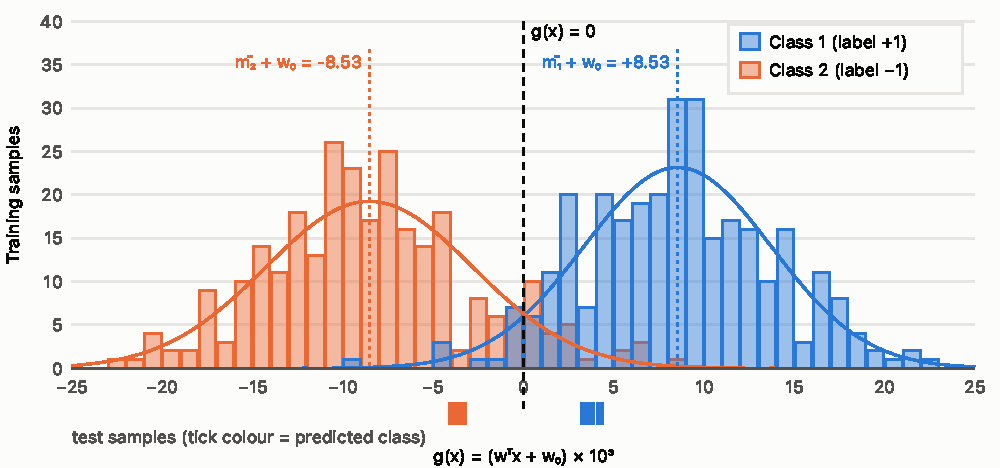
\includegraphics[width=\linewidth]{figures/fig2.pdf}
\caption{Training samples projected onto the Fisher direction, with a histogram of
$g(\mathbf{x}) = \mathbf{w}^T\mathbf{x} + w_0$ per class (bin width $1\times10^{-3}$) and the fitted 1-D Gaussians drawn over
them. The heavy dashed line is the boundary $g = 0$, the thin dotted lines mark the projected class means shifted by the bias, $\tilde{m}_1 + w_0$ and
$\tilde{m}_2 + w_0$, at $\pm 8.53\times10^{-3}$, and the ticks below the axis are the 23 test samples.}
\label{fig:fisher}
\end{figure}
